\documentclass{beamer}
\usepackage[T1,T2A]{fontenc}
\usepackage[utf8]{inputenc}
\usepackage[english,russian]{babel}
\usepackage{amsmath}
\usepackage{graphicx}
\usepackage{listings}
\usepackage{xcolor}

\usetheme{Madrid}
\definecolor{mygreen}{RGB}{0, 100, 100} 

\setbeamercolor{structure}{fg=mygreen} 
\setbeamercolor{palette primary}{fg=white, bg=mygreen} 
\setbeamercolor{titlelike}{fg=white, bg=mygreen} 
\setbeamercolor{block title}{fg=white, bg=mygreen} 

\title[КТА]{Краткая теория алгоритмов}
\author{Салимли Айзек}
\institute{MathLang}
\date{\today}
\newenvironment{rusdefinition}[1][Определение]{
    \begin{block}{#1}
}{\end{block}}
\newenvironment{rexample}[1][Пример]{\begin{exampleblock}{#1}}{\end{exampleblock}}

\lstset{
    language=Haskell,
    basicstyle=\ttfamily\small,
    inputencoding=utf8,
    extendedchars=true,
    literate={�}{{\bfseries?}}1 {^^ff}{{\bfseries?}}1,
    breaklines=true,
    breakatwhitespace=true,
    tabsize=2,
    frame=single
}

\begin{document}

\begin{frame}
    \titlepage
\end{frame}

\AtBeginSection[]{
    \begin{frame}{Содержание}
        \tableofcontents[currentsection]
    \end{frame}
}

\section{Конечный автомат}
\begin{frame}{Конечный автомат}

Конечный автомат - это формальная математическая модель, она легко описывает базовый принцип работы парсеров/ компиляторов/ анализаторов. 
\textcolor{red}{Это только математическая модель, которая легко реализовывается в коде}. \\
\begin{rusdefinition}
Формально это кортеж состоящий из:
\begin{itemize}
    \item Множество состояний - $S$
    \item Множество входного и выходного алфавита - $X, Y$ 
    \item Начальное состояние - $s_0$
    \item Функция переходов - $\delta : X \rightarrow S$
    \item Функция выходов - $\lambda : X \rightarrow Y$ 
\end{itemize}
\end{rusdefinition}
То есть DFA (Deterministic Finite Automaton): 
\[ DFA = (S, X, Y, s_0, \delta, \lambda) \]
\end{frame}

\begin{frame}{Конечный автомат}
    \begin{rexample}
    Возьмем в пример базовый турникет. \\
    Тут: 
    \[ DFA_{tourniquet} = (S = \{ goToMetro, lock, unlock\}, s_0 = \{goToMetro\}, X = \]
    \[ = \{push, coin\}, Y = \{unlock, lock\}, \delta = \{ push, coin\} \rightarrow \{lock, unlock\}, \lambda = \]
    \[ = \{ push, coin\} \rightarrow \{ lock, unlock \}) \]
        \begin{centering}
            \includegraphics[scale=0.45]{images/Mura.png}
        \end{centering}
    \end{rexample}
\end{frame}

\begin{frame}{Конечный автомат}
    \begin{rexample}
    Более сложный пример: автомат распазнает ссылку на яндекс диск:
    \begin{center}
        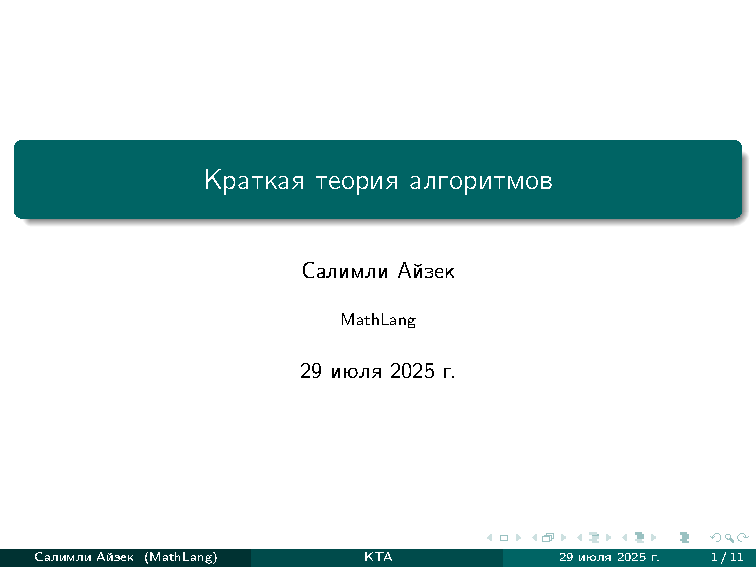
\includegraphics[scale=0.13]{images/DFA.png}
    \end{center}
\end{rexample}
\end{frame}

\subsection{Обозначения}
\begin{frame}{Обозначения}
\begin{itemize}
    \item Стартовое состояние - \includegraphics[scale = 0.4]{images/start.png}. 
    \item Переход из состояния в состояние - \includegraphics[scale = 0.4]{images/goTo.png}.
    \item Узел в то же состояние - \includegraphics[scale = 0.4]{images/inSameState.png}. 
    \item Финальное состояние - \includegraphics[scale = 0.4]{images/final.png}.  
\end{itemize}
\end{frame}


\section{Автоматы Мили и Мура}
\begin{frame}{Автоматы Мили и Мура}
    Существует два основных типа задания графического автомата: 
    \begin{itemize}
        \item К.А. Мили
        \item К.А. Мура  
    \end{itemize}
    \begin{rusdefinition}
    Автомат Мили и автомат Мура с одинаковой формальной структурой (кортежом) равносильны.
    Они отличаются лишь графически. При этом всегда можно перейти с автомата Мура в автомат Мили и наобарот. 
    \[ DFA_{Mili} = DFA_{Mura} \]  
\end{rusdefinition}
\end{frame}

\subsection{Автомат Мили}
\begin{frame}{Автомат Мили}
    \begin{center}
        \includegraphics[scale=0.5]{images/Mili.png}
    \end{center}
\end{frame}

\subsection{Автомат Мура}
\begin{frame}{Автомат Мура}
    \begin{center}
        \includegraphics[scale=0.5]{images/Mura.png}
    \end{center}
\end{frame}

\begin{frame}{}
    \centering
    \Large Спасибо за внимание!
    
    \vspace{1cm}
    \small \textcolor{red}{Пишите вопросы в комментариях!!!}
\end{frame}

\end{document}